\documentclass{article}
\usepackage{minted}
\usepackage{listings}
\usepackage{graphicx}
\usepackage{physics}
\usepackage{siunitx}
\usepackage{placeins}
\usepackage{hyperref}

\usepackage{lmodern}
\usepackage{amssymb,amsmath}
\usepackage{ifxetex,ifluatex}
\usepackage{fixltx2e} % provides \textsubscript
\ifnum 0\ifxetex 1\fi\ifluatex 1\fi=0 % if pdftex
  \usepackage[T1]{fontenc}
  \usepackage[utf8]{inputenc}
  \usepackage{textcomp} % provides euro and other symbols
\else % if luatex or xelatex
  \usepackage{unicode-math}
  \defaultfontfeatures{Ligatures=TeX,Scale=MatchLowercase}
\fi
% use upquote if available, for straight quotes in verbatim environments
\IfFileExists{upquote.sty}{\usepackage{upquote}}{}
% use microtype if available
\IfFileExists{microtype.sty}{%
\usepackage[]{microtype}
\UseMicrotypeSet[protrusion]{basicmath} % disable protrusion for tt fonts
}{}
\IfFileExists{parskip.sty}{%
\usepackage{parskip}
}{% else
\setlength{\parindent}{0pt}
\setlength{\parskip}{6pt plus 2pt minus 1pt}
}
\usepackage{hyperref}
\hypersetup{
            pdfborder={0 0 0},
            breaklinks=true}
\urlstyle{same}  % don't use monospace font for urls
\usepackage{color}
\usepackage{fancyvrb}
\newcommand{\VerbBar}{|}
\newcommand{\VERB}{\Verb[commandchars=\\\{\}]}
\DefineVerbatimEnvironment{Highlighting}{Verbatim}{commandchars=\\\{\}}
% Add ',fontsize=\small' for more characters per line
\newenvironment{Shaded}{}{}
\newcommand{\AlertTok}[1]{\textcolor[rgb]{1.00,0.00,0.00}{\textbf{#1}}}
\newcommand{\AnnotationTok}[1]{\textcolor[rgb]{0.38,0.63,0.69}{\textbf{\textit{#1}}}}
\newcommand{\AttributeTok}[1]{\textcolor[rgb]{0.49,0.56,0.16}{#1}}
\newcommand{\BaseNTok}[1]{\textcolor[rgb]{0.25,0.63,0.44}{#1}}
\newcommand{\BuiltInTok}[1]{#1}
\newcommand{\CharTok}[1]{\textcolor[rgb]{0.25,0.44,0.63}{#1}}
\newcommand{\CommentTok}[1]{\textcolor[rgb]{0.38,0.63,0.69}{\textit{#1}}}
\newcommand{\CommentVarTok}[1]{\textcolor[rgb]{0.38,0.63,0.69}{\textbf{\textit{#1}}}}
\newcommand{\ConstantTok}[1]{\textcolor[rgb]{0.53,0.00,0.00}{#1}}
\newcommand{\ControlFlowTok}[1]{\textcolor[rgb]{0.00,0.44,0.13}{\textbf{#1}}}
\newcommand{\DataTypeTok}[1]{\textcolor[rgb]{0.56,0.13,0.00}{#1}}
\newcommand{\DecValTok}[1]{\textcolor[rgb]{0.25,0.63,0.44}{#1}}
\newcommand{\DocumentationTok}[1]{\textcolor[rgb]{0.73,0.13,0.13}{\textit{#1}}}
\newcommand{\ErrorTok}[1]{\textcolor[rgb]{1.00,0.00,0.00}{\textbf{#1}}}
\newcommand{\ExtensionTok}[1]{#1}
\newcommand{\FloatTok}[1]{\textcolor[rgb]{0.25,0.63,0.44}{#1}}
\newcommand{\FunctionTok}[1]{\textcolor[rgb]{0.02,0.16,0.49}{#1}}
\newcommand{\ImportTok}[1]{#1}
\newcommand{\InformationTok}[1]{\textcolor[rgb]{0.38,0.63,0.69}{\textbf{\textit{#1}}}}
\newcommand{\KeywordTok}[1]{\textcolor[rgb]{0.00,0.44,0.13}{\textbf{#1}}}
\newcommand{\NormalTok}[1]{#1}
\newcommand{\OperatorTok}[1]{\textcolor[rgb]{0.40,0.40,0.40}{#1}}
\newcommand{\OtherTok}[1]{\textcolor[rgb]{0.00,0.44,0.13}{#1}}
\newcommand{\PreprocessorTok}[1]{\textcolor[rgb]{0.74,0.48,0.00}{#1}}
\newcommand{\RegionMarkerTok}[1]{#1}
\newcommand{\SpecialCharTok}[1]{\textcolor[rgb]{0.25,0.44,0.63}{#1}}
\newcommand{\SpecialStringTok}[1]{\textcolor[rgb]{0.73,0.40,0.53}{#1}}
\newcommand{\StringTok}[1]{\textcolor[rgb]{0.25,0.44,0.63}{#1}}
\newcommand{\VariableTok}[1]{\textcolor[rgb]{0.10,0.09,0.49}{#1}}
\newcommand{\VerbatimStringTok}[1]{\textcolor[rgb]{0.25,0.44,0.63}{#1}}
\newcommand{\WarningTok}[1]{\textcolor[rgb]{0.38,0.63,0.69}{\textbf{\textit{#1}}}}
\setlength{\emergencystretch}{3em}  % prevent overfull lines
\providecommand{\tightlist}{%
  \setlength{\itemsep}{0pt}\setlength{\parskip}{0pt}}
\setcounter{secnumdepth}{0}
% Redefines (sub)paragraphs to behave more like sections
\ifx\paragraph\undefined\else
\let\oldparagraph\paragraph
\renewcommand{\paragraph}[1]{\oldparagraph{#1}\mbox{}}
\fi
\ifx\subparagraph\undefined\else
\let\oldsubparagraph\subparagraph
\renewcommand{\subparagraph}[1]{\oldsubparagraph{#1}\mbox{}}
\fi

% set default figure placement to htbp
\makeatletter
\def\fps@figure{htbp}
\makeatother

\graphicspath{{../figures/}}

\begin{document}
    \begin{center}
        \Large AMATH 582 Final: Predicting Remaining Useful Life of Li-Ion
        Batteries from Discharge Profiles \par
        \large Brady Griffith
    \end{center}

    \begin{abstract}
        Li-Ion batteries are an important tool for scientific instrumentation,
        but their capacity decreases as they are used. In this project, A
        reduced dimensional basis is found though SVD to represent the discharge
        curves in. A linear regression is then used to predict the capacity
        remaining. In test data, not part of the training, the correct capacity
        is consistently found within $2 \%$ capacity.
    \end{abstract}

    \section{Introduction and Overview}
    Li-ion batteries are everywhere. They're in almost every modern
    electronic device: smartphones, headphones, and electric cars. But my
    personal interest is in their application to scientific payloads.
    Satellites and balloons wouldn't be able to operate on the dark side
    of the earth without these batteries. They are often exposed to conditions
    worse than even the most reckless phone owner can concoct. And if you
    recover these batteries, as is often possible for balloon flights, I'd like
    to know if these batteries still have life left.

    For this analysis, I'm using a dataset from the NASA Ames Research Center.
    \cite{bat_data}
    Four 18650 sized Li-ion were repeatedly discharged and recharged with the
    voltage and current being recorded. This cycle was repeated until each
    battery had lost 30 \% of its original capacity. This dataset also includes
    Electrochemical Impedance Spectroscopy analysis, which I will ignore, since
    I've never worked in a lab with an instrument that makes that measurement
    and wouldn't have much use for it to make predictions.

    Because of their prevalence, there is a lot of literature on indicators of
    battery health. I am deliberately ignoring this, because I would like this
    project have more of a focus on the analysis techniques that can apply to
    systems that have been less well characterized.

    \section{Theoretical Background}
    % Electricity basics needed
    Some basic electrical theory is needed to understand how I reworked the
    discharge curves to be more general. In the data set, the measurements
    are presented as time series of voltage and current. If I used them as is,
    I couldn't apply the results to a system that takes a similar measurement,
    but with a different constant current or a constant discharge resistance
    (which is what my undergrad lab's battery characterizer used.) It also
    wouldn't generalize to larger capacity lithium ion batteries. Instead, I
    would like to preform the analysis on the voltage as a function of the
    percentage discharge.

    The power consumed from a battery can be found from the current,$I(t)$, and
    voltage, $V(t)$.
    by
    $$ P(t) = I(t)V(t) $$
    The power consumed from the start at $t_0$ up to a time $t$ is given by
    $$ W(t) = \int_{t_0}^t P(t^\prime) \dd{t^\prime}$$
    If the battery is fully discharged by $t_f$, the fraction discharged $C(t)$
    is then
    $$ C(t) = W(t)/W(t_f) $$
    I also define a remaining capacity value for curve $i$ defined to be
    \begin{equation}
            R_i \equiv C_i(t_f) / C_{\max}(t_f)
    \end{equation}

    With the curves expressed in terms of a preferred independent variable, I
    can now reduce the dimensionality of the system through SVD. The discharge
    curves all have the same general shape, with some changes occurring as they
    age (See figure \ref{fig:curves_aging}). For this reason I would expect the
    system to represented well by a fairly low dimension system.

    \begin{figure}[tbp]
        \centering
        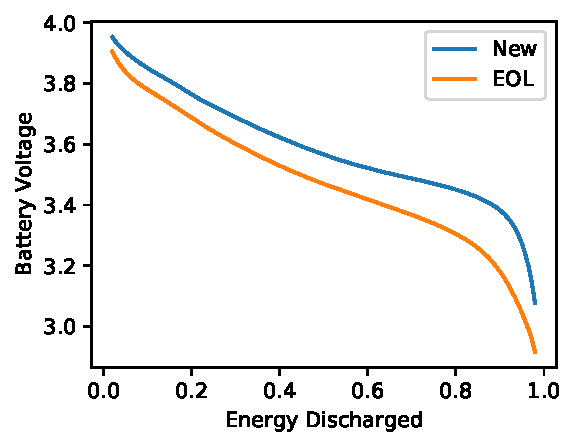
\includegraphics[width=.7\textwidth]{aging_curves.pdf}
        \caption{\label{fig:curves_aging} Two example discharge curves for
        Battery 5. One curve is a new battery with full capacity and the
        second is at the battery end of life (EOL) when it has lost $30\%$
        of its starting capacity.}
    \end{figure}

    % Model
    Looking at these changes to the discharge curve (see figure
    \ref{fig:svd_proj}), the leading order terms can by expressed as a linear
    function of the aging. This model can be written out
    \begin{equation}
        R = \frac{1}{k}
            \sum_i^k a_i x_i + b_i
    \end{equation}

    \begin{figure}[tbp]
        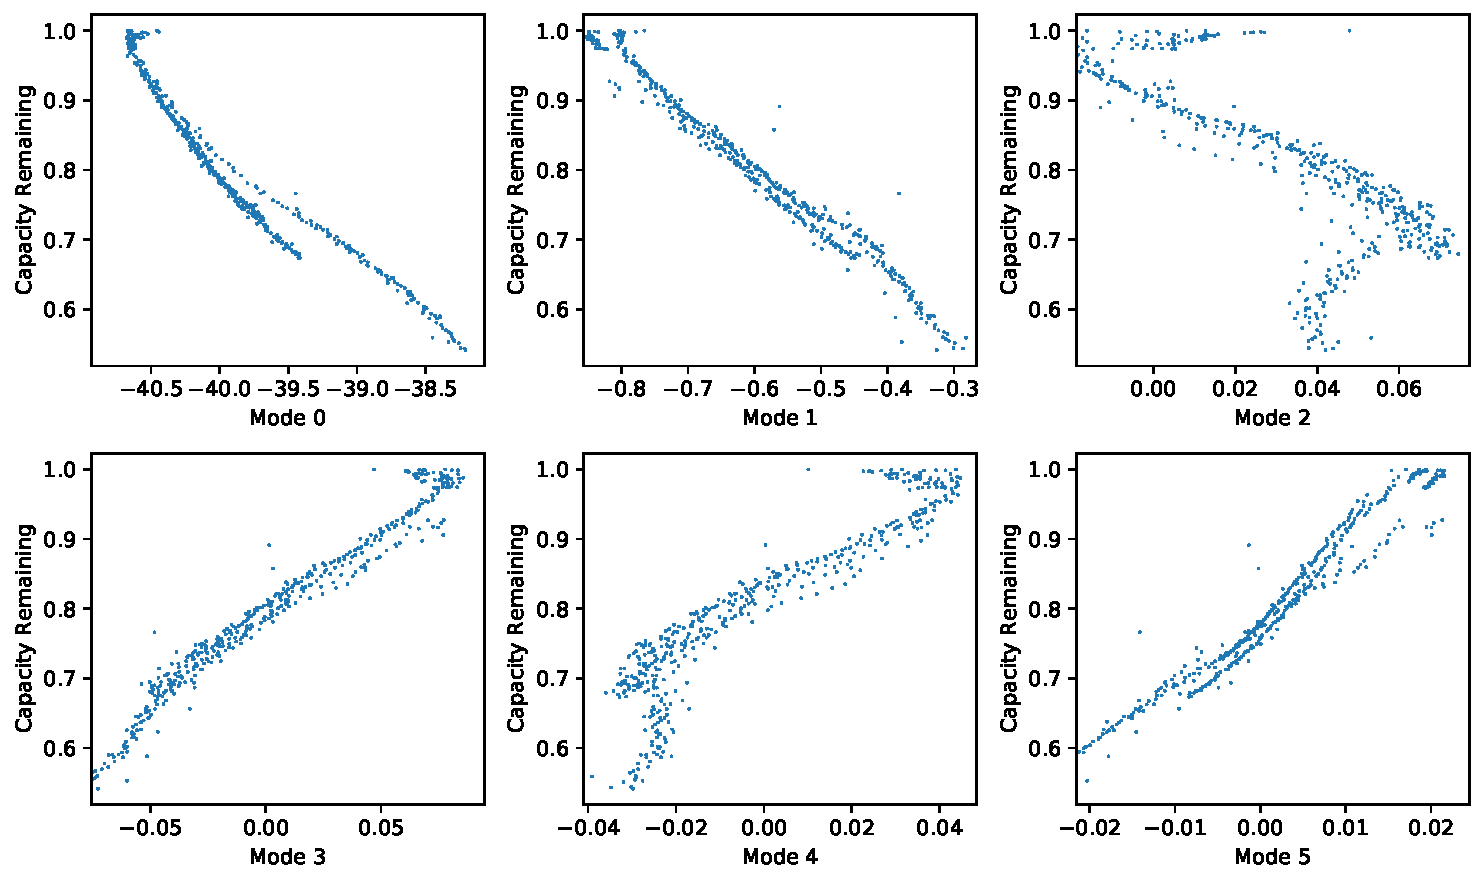
\includegraphics[width=\textwidth]{mode_proj.pdf}
        \caption{\label{fig:svd_proj} A scatter plot of how the battery
        capacity changes with the first 6 SVD modes. This has been cropped
        to highlight main distribution, so there are outliers not shown.}
    \end{figure}

    \begin{equation}
        \vb{R} = \begin{bmatrix}
            \vb{x_0} & 1 \\ \vb{x_1} & 1 \\ \vdots & \vdots \\ \vb{x_m} & 1
        \end{bmatrix}
        \begin{bmatrix}
            a_0/k \\
            a_1/k \\
            \vdots \\
            a_k/k \\
            \frac{1}{k} \sum_i^k b_i
        \end{bmatrix}
    \end{equation}

    \begin{equation*}
        \vb{R} = \vb{X} \vb{b}
    \end{equation*}

    Which is now a regression problem and can be solved least squares or any
    of the different norm methods discussed in chapter 18 of the book
    \cite{Kutz2013}.

    \section{Algorithm Implementation and Development}
    % Interpolation
    Generality to other batteries and discharge curve recorders is a major
    objective in my analysis, so I would like to put the curves into a form
    independent of the sampling rate. After calculating $C(t)$ for each
    recording, I define linearly spaced set of 128 points over
    $C(t) = (.02, .98)$. The first and last $2 \%$ were ignored because battery
    voltages bounce back after the load is removed, and that is not part of this
    analysis.

    I preform the model fitting using the curves from batteries 5, 6, and 7.
    Battery 18 is reserved for testing. The regression used here was least
    squares. There are outlier, so it may have benefitted from use of a
    Lasso regression instead.

    \section{Computational Results}
    % SVD Modes
    First, I need to determine the how many SVD modes are needed. In figure
    \ref{fig:mode_frac} I plot the fraction of total covariance in $n$ modes.
    20 modes excluded $< 10^6 $ of total covariance and visually recreates the
    curve to a subjectively good quality.
    \begin{figure}[tbp]
        \centering
        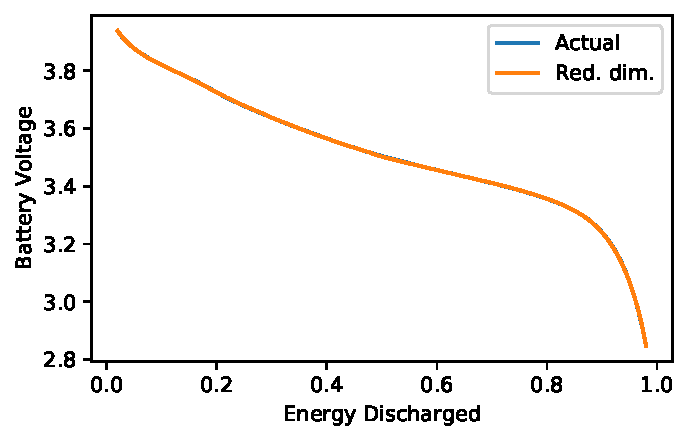
\includegraphics[width=.48\textwidth]{red_dim.pdf}
        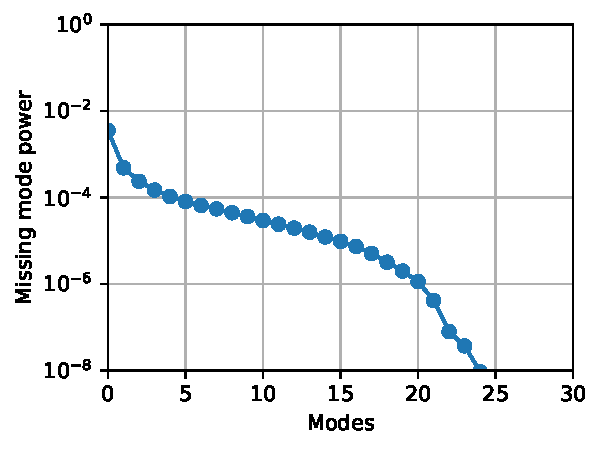
\includegraphics[width=.48\textwidth]{mode_frac.pdf}
        \caption{\label{fig:mode_frac} On the right, fraction of variance
        contained in $n$ svd modes. On the left, an example discharge curve
        represented by 20 modes.}
    \end{figure}

    The weights for the model is found. The predicted values for the training
    set consistently fall within a range of $2 \%$ capacity remaining. The
    performance on the battery not used in the training data is slightly worse,
    but still . See the distribution in figure \ref{fig:model_dist}.

    \begin{figure}[tbp]
        \centering
        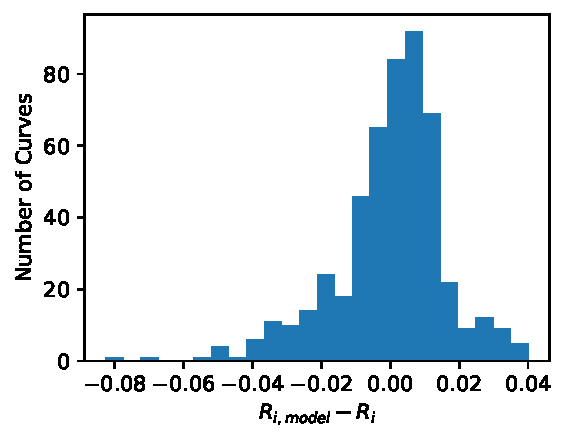
\includegraphics[width=.48\textwidth]{train-pref.pdf}
        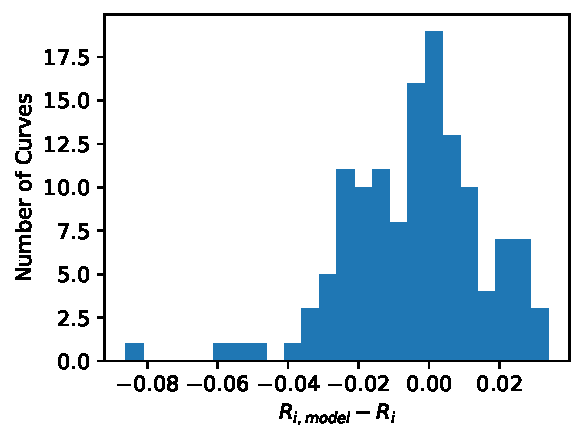
\includegraphics[width=.48\textwidth]{test-pref.pdf}
        \caption{\label{fig:model_dist} On the left, the distribution of
        errors for the model with the training data. On the right with the
        test data.}
    \end{figure}

    \section{Summary and Conclusions}
    % Did it work
    In this project, SVD was first used create an ideal basis to represent
    Li-Ion discharge curves. Then once in this basis, a linear regression is
    to determine the battery capacity, and thus remaining life. For the test
    data, not part of the training, the regression could accurately predict the
    capacity an error $\pm 2 \% $ capacity. This would accurate enough to make
    decisions about when a battery needs to be replaced.

    % Future work - other batteries
    Another test that wasn't performed for this project, but that would be an
    important next step is checking how well these results generalize to
    another lithium ion battery. I have a couple discharge curves saved from
    an undergrad lightning ballooning project that could have been used for
    this.
    
    \bibliographystyle{ieeetr}
    \bibliography{bibliography}

    \FloatBarrier
    \newpage
    \appendix
    Here is a \href{https://github.com/bagriffith/AMATH582/tree/main/Final}
    {link to the Github repository for this project}.
    \section{Python Functions}
    % Use PyDoc to generate
    \subsection{dmd}

\subsubsection{dmd}

\begin{Shaded}
\begin{Highlighting}[]
\NormalTok{dmd(X2, u, s, vh)}
\end{Highlighting}
\end{Shaded}

Returns the DMD modes and complex frequencies for the system.

\textbf{Arguments}:

\begin{itemize}
\tightlist
\item
  \texttt{X2} \emph{array-like} - The X\_2\^{}M matrix
\item
  \texttt{u} \emph{array-like} - The U matrix of the X\_1\^{}M-1 SVD
\item
  \texttt{s} \emph{array-like} - The s array of the X\_1\^{}M-1 SVD
\item
  \texttt{vh} \emph{array-like} - The vh matrix of the X\_1\^{}M-1 SVD
\end{itemize}

\textbf{Returns}:

\begin{itemize}
\tightlist
\item
  \texttt{ndarray} - Array of complex frequencies for DMD modes
\item
  \texttt{ndarray} - Matrix with rows of the DMD modes
\end{itemize}

\subsubsection{x\_dmd}

\begin{Shaded}
\begin{Highlighting}[]
\NormalTok{x_dmd(t, psi, w, b)}
\end{Highlighting}
\end{Shaded}

The DMD approximation of x(t).

\textbf{Arguments}:

\begin{itemize}
\tightlist
\item
  \texttt{t} \emph{float} - The time in frames
\item
  \texttt{psi} \emph{array-like} - Matrix with rows of the DMD modes
\item
  \texttt{w} \emph{array-like} - Array of complex frequencies for DMD
  modes
\item
  \texttt{b} \emph{array-like} - Array of initial values of the DMD
  modes
\end{itemize}

\textbf{Returns}:

\begin{itemize}
\tightlist
\item
  \texttt{ndarray} - DMD approximation of pixels at t
\end{itemize}

\subsubsection{frame\_bg\_sep}

\begin{Shaded}
\begin{Highlighting}[]
\NormalTok{frame_bg_sep(t, X, psi, w, b)}
\end{Highlighting}
\end{Shaded}

Separate the forground and background of frame t

\textbf{Arguments}:

\begin{itemize}
\tightlist
\item
  \texttt{t} \emph{int} - The time in frames
\item
  \texttt{psi} \emph{array-like} - Matrix with rows of the DMD modes
\item
  \texttt{w} \emph{array-like} - Array of complex frequencies for DMD
  modes
\item
  \texttt{b} \emph{array-like} - Array of initial values of the DMD
  modes
\end{itemize}

\textbf{Returns}:

\begin{itemize}
\tightlist
\item
  \texttt{ndarray} - Foreground array
\item
  \texttt{ndarray} - Background array
\end{itemize}

\subsubsection{show\_frame}

\begin{Shaded}
\begin{Highlighting}[]
\NormalTok{show_frame(frame, shape, path_out)}
\end{Highlighting}
\end{Shaded}

Plot the frame provided.

\textbf{Arguments}:

\begin{itemize}
\tightlist
\item
  \texttt{frame} \emph{array-like} - 1 D array of pixels
\item
  \texttt{shape} \emph{tuple} - The shape of the image (pixels\_y,
  pixels\_x)
\item
  \texttt{path\_out} \emph{str} - Path to save figure to
\end{itemize}

\subsection{svd}

\subsubsection{plot\_n\_modes}

\begin{Shaded}
\begin{Highlighting}[]
\NormalTok{plot_n_modes(X, V, n, shape, path_out)}
\end{Highlighting}
\end{Shaded}

Shows the numbers represented with the selected number of SVD modes

\textbf{Arguments}:

\begin{itemize}
\tightlist
\item
  \texttt{X} \emph{array\_like} - Data matrix with rows of images
\item
  \texttt{V} \emph{array\_like} - Matrix with mode vectors as columns
\item
  \texttt{n} \emph{int} - Number of modes to use in the representation
\item
  \texttt{shape} \emph{tuple} - The shape of the image (pixels\_y,
  pixels\_x)
\item
  \texttt{path\_out} \emph{str} - Path to save figure to
\end{itemize}

\subsubsection{plot\_mode\_fraction}

\begin{Shaded}
\begin{Highlighting}[]
\NormalTok{plot_mode_fraction(s, path_out)}
\end{Highlighting}
\end{Shaded}

Plots the fraction of power represented with n modes

\textbf{Arguments}:

\begin{itemize}
\tightlist
\item
  \texttt{s} \emph{array-like} - 1D arrray of the variances of the
  principal components.
\item
  \texttt{path\_out} \emph{str} - Path to save figure to
\end{itemize}

\subsection{loadVid}

\subsubsection{open\_video}

\begin{Shaded}
\begin{Highlighting}[]
\NormalTok{open_video(vid_path)}
\end{Highlighting}
\end{Shaded}

Loads the video matrices

\textbf{Arguments}:

\begin{itemize}
\tightlist
\item
  \texttt{vid\_path} \emph{str} - Path to the video file
\end{itemize}

\textbf{Returns}:

\begin{itemize}
\tightlist
\item
  \texttt{ndarray} - X\_1\^{}M-1
\item
  \texttt{ndarray} - X\_2\^{}M
\end{itemize}


    \section{Python Code}
    \subsection{main.py}
    \inputminted{python}{../code/main.py}

    \subsection{loadCurves.py}
    \inputminted{python}{../code/loadCurves.py}

    \subsection{svd.py}
    \inputminted{python}{../code/svd.py}

    \subsection{predict.py}
    \inputminted{python}{../code/predict.py}

\end{document}
